\section{Reti Wireless e Mobili}
Questo capitolo introduce due sfide distinte: le reti \textit{wireless} (che gestiscono l'inaffidabilità del mezzo radio) e le reti \textit{mobili} (che gestiscono gli utenti che cambiano il loro punto di connessione alla rete).

\noindent Gli elementi chiave di una rete wireless sono:
\begin{itemize}
    \item \textbf{Host wireless:} I dispositivi finali (laptop, smartphone).
    \item \textbf{Collegamenti wireless:} Il mezzo fisico (radio) usato per connettere gli host.
    \item \textbf{Stazione Base (Base Station):} L'infrastruttura di rete che si connette alla rete cablata più grande. Nelle reti WiFi è chiamata \textbf{Access Point (AP)}, nelle reti cellulari è la \textbf{stazione radio base} (o eNodeB in 4G).
\end{itemize}
Le reti che utilizzano una stazione base operano in \textbf{modalità infrastruttura} (infrastructure mode). Le reti senza un'entità centrale (es. Bluetooth) operano in \textbf{modalità ad-hoc}.

\subsection{Caratteristiche dei collegamenti wireless}
I collegamenti radio sono molto diversi dai cavi:
\begin{itemize}
    \item \textbf{Attenuazione del segnale (Path Loss):} Il segnale si indebolisce con la distanza.
    \item \textbf{Interferenza:} Altre sorgenti che trasmettono sulla stessa frequenza (es. microonde, altri AP) creano "rumore".
    \item \textbf{Propagazione Multipath:} Il segnale radio rimbalza su oggetti (muri, palazzi) e arriva al ricevitore tramite percorsi multipli, che possono interferire distruttivamente tra loro.
\end{itemize}
Questi fattori causano un \textbf{Bit Error Rate (BER)} molto più alto rispetto ai cavi.

\subsubsection{Il Problema del Terminale Nascosto}
Questa è una sfida fondamentale delle reti wireless. Come mostrato nella figura, l'Host A e l'Host C sono entrambi nel raggio della Stazione Base B, ma non sono nel raggio l'uno dell'altro.
\begin{itemize}
    \item Se A sta trasmettendo a B, C non può sentirlo.
    \item Se C decide di trasmettere (pensando che il canale sia libero), la sua trasmissione causerà una \textbf{collisione} \textit{presso il ricevitore} (B).
    \item A e C non sapranno mai che la collisione è avvenuta, perché non possono rilevarla.
\end{itemize}
Questo problema rende il protocollo CSMA/CD di Ethernet (Collision \textit{Detection}) inutilizzabile nel wireless.

\begin{center}
    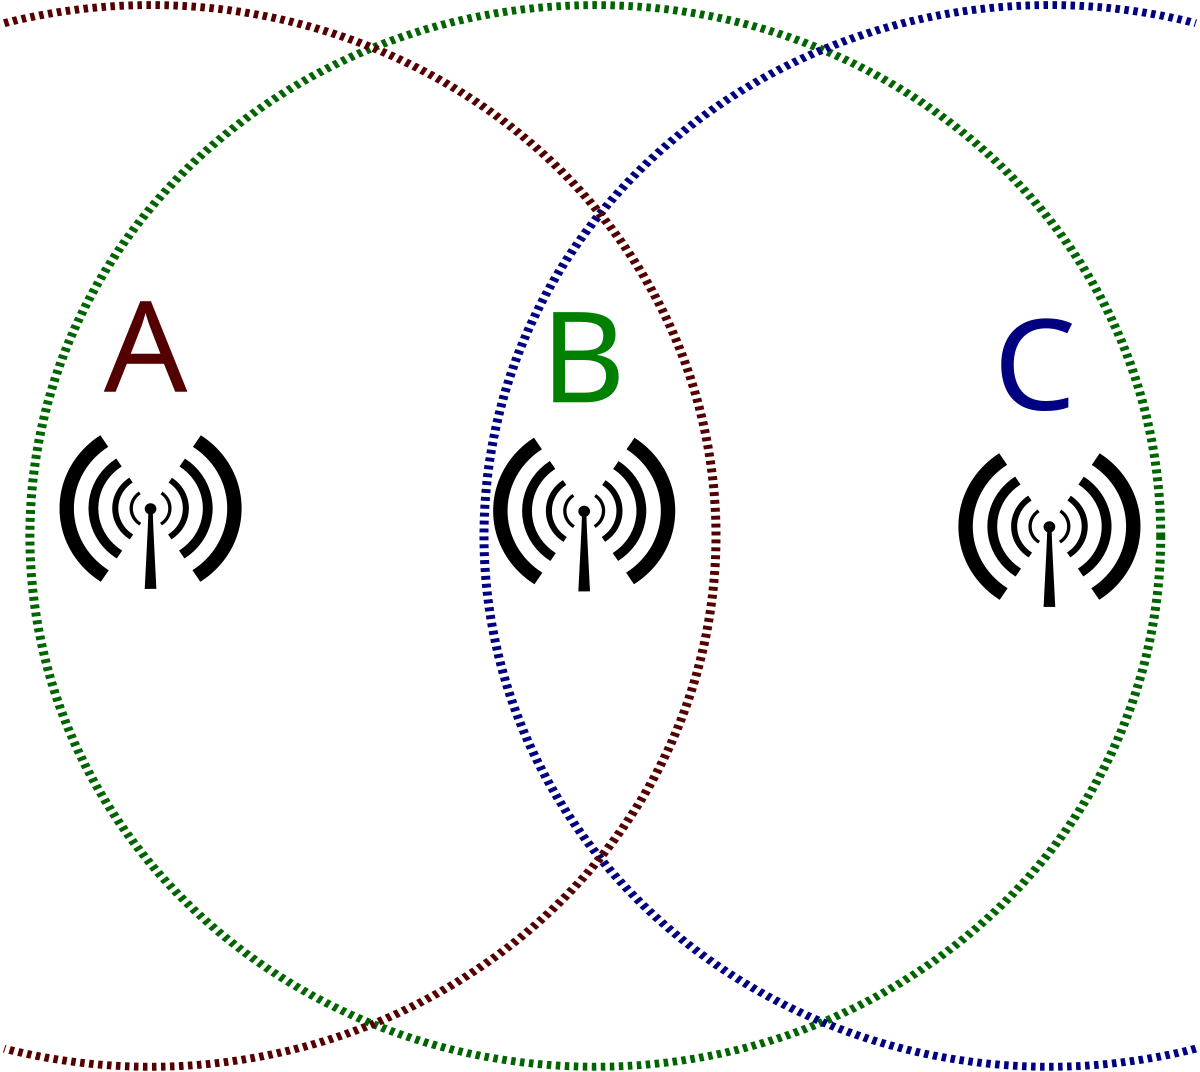
\includegraphics[width=0.6\textwidth]{img/hidden_terminal_problem.png}
\end{center}

\subsection{WiFi: Reti LAN 802.11}

\subsubsection{Architettura 802.11}
L'unità fondamentale è il \textbf{Basic Service Set (BSS)}. Consiste in uno o più host wireless e un \textbf{Access Point (AP)} centrale, che li collega alla rete cablata (es. a uno switch Ethernet).

\textbf{Associazione all'AP:}
Prima di inviare dati, un host deve "associarsi" a un AP.
\begin{enumerate}
    \item \textbf{Scoperta (Scanning):} L'host trova gli AP disponibili.
        \begin{itemize}
            \item \textbf{Scansione Passiva:} L'host ascolta passivamente i \textbf{beacon frame} (frame "faro") che ogni AP trasmette periodicamente. Il beacon contiene l'SSID (il nome della rete, es. "TIM-12345") e l'indirizzo MAC dell'AP.
            \item \textbf{Scansione Attiva:} L'host trasmette un \textit{Probe Request frame} in broadcast. Tutti gli AP in portata rispondono con un \textit{Probe Response frame}.
        \end{itemize}
    \item \textbf{Autenticazione e Associazione:} L'host sceglie un AP (di solito quello con il segnale più forte) e completa un processo di richiesta/risposta di associazione (\textit{Association Request/Response}).
    \item \textbf{DHCP:} Una volta associato, l'host usa DHCP (come su una rete cablata) per ottenere un indirizzo IP dall'AP.
\end{enumerate}

\subsubsection{Il protocollo MAC 802.11: CSMA/CA}
Poiché la \textit{rilevazione} delle collisioni (CD) non è fattibile, 802.11 usa la \textbf{Prevenzione} \textit{delle collisioni} (\textbf{CSMA/CA} - Collision Avoidance).

\textbf{Funzionamento:}
\begin{itemize}
    \item \textbf{ACK di Livello Collegamento:} Dato che i link wireless sono inaffidabili, ogni frame dati \textit{deve} essere confermato da un \textbf{ACK} (acknowledgment) di livello 2. Se il mittente non riceve l'ACK dopo un breve tempo (SIFS), assume che il frame sia andato perso (per collisione o errore) e lo \textbf{ritrasmette} dopo un backoff.
    \item \textbf{CSMA/CA:}
        \begin{enumerate}
            \item Ascolta il canale (Carrier Sense).
            \item Se il canale è libero per un tempo (DIFS), trasmette il frame.
            \item Se il canale è occupato, sceglie un tempo di \textbf{backoff} casuale e avvia un contatore.
            \item Il contatore scende solo quando il canale è libero. Quando arriva a zero, l'host trasmette.
        \end{enumerate}
    \item \textbf{RTS/CTS (Opzionale):} Per mitigare il problema del terminale nascosto, un host può inviare un breve frame \textbf{RTS} (Request To Send). L'AP risponde con un \textbf{CTS} (Clear To Send). Il CTS viene sentito da tutti i nodi nel raggio dell'AP (incluso il terminale nascosto), che sanno di dover tacere per la durata indicata nel frame.
\end{itemize}

\subsection{Reti Cellulari: Architettura 4G/5G}
Le reti cellulari sono progettate per la mobilità su vasta area. L'architettura 4G \textbf{LTE (Long-Term Evolution)} è un'architettura \textit{all-IP}.

L'architettura 4G si divide in due parti principali:
\begin{description}
    \item[Radio Access Network (RAN):] È la parte "radio". Contiene le stazioni base (chiamate \textbf{eNodeB}) che gestiscono il collegamento wireless con i dispositivi mobili (chiamati \textbf{UE} - User Equipment).
    \item[Evolved Packet Core (EPC):] È il "cervello" e la "dorsale" (core) dell'operatore telefonico. Collega tutte le stazioni radio RAN a Internet.
\end{description}

\subsubsection{Componenti Chiave dell'EPC (Core 4G)}
L'EPC è diviso in un \textbf{Piano di Dati} (per il traffico utenti) e un \textbf{Piano di Controllo} (per la gestione della rete).

\textbf{Elementi del Piano di Controllo:}
\begin{itemize}
    \item \textbf{HSS (Home Subscriber Server):} È il database principale dell'operatore. Contiene i profili di tutti i suoi abbonati: il loro identificativo univoco (IMSI), i servizi a cui hanno diritto (es. 4G, 5G, chiamate internazionali) e le chiavi segrete per l'autenticazione. Si trova solo nella rete \textit{home} dell'utente.
    \item \textbf{MME (Mobility Management Entity):} È il "cervello" della rete. Gestisce la \textbf{mobilità}: autentica gli utenti (parlando con l'HSS), gestisce l'aggancio (attach) alla rete e, soprattutto, \textbf{traccia la posizione} (handoff) dell'utente (a quale eNodeB è connesso in un dato momento).
\end{itemize}

\textbf{Elementi del Piano Dati:}
\begin{itemize}
    \item \textbf{S-GW (Serving Gateway):} È il punto di "ancoraggio" per la mobilità all'interno della RAN. Tutto il traffico dati dell'utente (UE) passa attraverso l'S-GW. Quando l'utente si sposta tra due eNodeB (handoff), l'S-GW non cambia, facilitando la transizione.
    \item \textbf{P-GW (PDN Gateway - Packet Data Network Gateway):} È il gateway che connette la rete dell'operatore a \textbf{Internet}. È il P-GW che \textbf{assegna l'indirizzo IP} al dispositivo mobile (spesso tramite NAT).
\end{itemize}

Il percorso dati utente è: \textbf{Mobile (UE)} $\leftrightarrow$ \textbf{eNodeB} $\leftrightarrow$ \textbf{S-GW} $\leftrightarrow$ \textbf{P-GW} $\leftrightarrow$ \textbf{Internet}.
Questo percorso tra gli elementi del core (eNodeB, S-GW, P-GW) è implementato usando \textbf{tunnel IP} (protocollo GTP).

\subsubsection{Cenni sul 5G}
Il 5G non è solo "4G più veloce". Introduce cambiamenti architetturali:
\begin{itemize}
    \item \textbf{Frequenze:} Utilizza frequenze molto più alte (\textit{millimeter wave}) che offrono banda larghissima ma hanno una portata molto più corta (richiedendo molte più "small cell").
    \item \textbf{Separazione Controllo/Dati (CUPS):} Il 5G separa in modo netto le funzioni del piano di controllo (gestite centralmente) da quelle del piano dati (che possono essere distribuite ai margini della rete, vicino all'utente), seguendo una logica simile a SDN.
    \item \textbf{Network Slicing:} Permette all'operatore di "affettare" la sua rete fisica in più reti virtuali logiche, ognuna ottimizzata per un servizio diverso (es. una "fetta" a bassa latenza per l'auto a guida autonoma, una "fetta" a banda larga per lo streaming video).
\end{itemize}

\subsection{Princìpi di Mobilità a Livello di Rete}
Come fa un server su Internet a inviare un pacchetto a un telefono che si muove nel mondo?

\subsubsection{Home Network e Visited Network (Roaming)}
Ogni dispositivo mobile ha una \textbf{Home Network} (es. TIM Italia), che è la rete del suo operatore (dove risiede il suo profilo HSS).
Quando un utente va all'estero (es. in Francia) e si connette a un operatore locale (es. Orange), quella è la \textbf{Visited Network} (rete visitata). Questo processo è chiamato \textbf{roaming}.
La rete visitata deve contattare la rete home per:
\begin{enumerate}
    \item Autenticare l'utente (tramite MME e HSS).
    \item Ottenere il permesso di fornire il servizio.
    \item Stabilire come instradare i pacchetti da e verso l'utente.
\end{enumerate}

\subsubsection{Routing Indiretto (Indirect Routing)}
Le reti mobili usano il routing indiretto per gestire il roaming.
Supponiamo che Alice (in Italia, rete home TIM) sia in roaming a New York (rete visitata AT&T) e che Bob (su un server a Roma) voglia inviarle un pacchetto.
\begin{enumerate}
    \item \textbf{Fase 1:} Bob invia il pacchetto all'indirizzo IP \textit{permanente} di Alice (che è un IP della rete TIM). I router di Internet instradano il pacchetto verso la rete home di Alice, cioè al P-GW di TIM in Italia.
    \item \textbf{Fase 2:} Il P-GW di TIM sa (grazie all'MME/HSS) che Alice si trova attualmente presso AT&T a New York.
    \item \textbf{Fase 3:} Il P-GW di TIM \textbf{incapsula} il pacchetto originale di Bob dentro un nuovo pacchetto IP (un tunnel). L'header di questo nuovo pacchetto ha come destinazione il P-GW (o S-GW) della rete AT&T a New York.
    \item \textbf{Fase 4:} Il gateway di AT&T riceve il pacchetto, lo "spacchetta" (decapsula) e consegna il pacchetto originale di Bob ad Alice.
\end{itemize}
Questo approccio crea il \textbf{Problema del Triangle Routing}: il traffico da Roma a New York (dove si trova Alice) deve prima viaggiare fino alla rete home (Italia), per poi essere re-instradato a New York (Roma $\rightarrow$ Italia $\rightarrow$ New York).

\subsubsection{Handoff (o Handover)}
L'Handoff (o Handover) è il processo che permette a un utente di spostarsi tra due celle (due eNodeB) \textit{senza interrompere la connessione} (es. durante una chiamata VoIP).

\textbf{Procedura (semplificata)}:
\begin{enumerate}
    \item L'UE misura continuamente la potenza del segnale della sua cella ("sorgente") e di quelle vicine ("target"). Quando il segnale della sorgente si indebolisce e quello di una target si rafforza, lo comunica alla sua stazione base (sorgente).
    \item La stazione base \textbf{sorgente} decide di avviare l'handoff. Contatta la stazione base \textbf{target} (tramite l'MME) e le chiede di allocare le risorse (canali radio) per l'UE in arrivo.
    \item La stazione target conferma e alloca le risorse.
    \item La stazione sorgente invia un comando all'UE: "Spostati alla stazione target (canale X, freq Y)".
    \item L'UE si sgancia dalla sorgente e si aggancia (associa) alla target.
    \item La stazione target informa l'MME, che a sua volta comanda all'\textbf{S-GW} (il punto di ancoraggio) di \textbf{cambiare il tunnel}: invece di inviare i pacchetti alla stazione sorgente, da ora deve inviarli alla stazione target.
    \item La stazione sorgente inoltra eventuali pacchetti arrivati in ritardo alla stazione target, per evitare perdite.
\end{enumerate}
L'intero processo è gestito dal piano di controllo (MME) ed è progettato per essere talmente veloce (millisecondi) da non essere percepito dall'utente.

